\subsubsection{Functional Requirements}
\begin{itemize}
  \item The system should apply a discount of 10\% on the last ride if it detects the user took at least two other passengers onto the car.
  \item The system should apply a discount of 20\% on the last ride if the car is left with no more than 50\% of the battery empty.
  \item The system should apply a discount of 30\% on the last ride If the car is left at special parking areas where they can be recharged and the user takes care of plugging the car into the power grid.
  \item The system should charge 30\% more n the last ride if a car is left at more then 3 KM from the nearest power grid station or with more than 80\% of the battery empty.
\end{itemize}

\subsubsection{Scenario 1}
Mark is a PowerEnJoy user. One day Jenny hang out with Tom. They decided to take a PowerEnJoy car for going in a club in the other side of the city. Mark is the only one with an account, so he reserves a car, unlocks it and drives. Near the club there is a \gls{charging station}, so he decides to go there to park the car. When he turns off the engine and they exit the car he also plugs the car into the power grid. After a while Mark receivs an e-mail from PowrEnJoy. He opens it and happily finds out that a discount of 30\% was applied on his last ride due to his virtuous behaviour.

\subsubsection{Scenario 2}
Susan decides to go to the supermarket with her sister and her mother. She knows that using PowerEnJoy there'is a discount of the 10\% the user took at least two other passengers onto the car. But when she arrives to the supermarket the battery of the car was 85\% empty. That is a problem, because the cost for re-charge the cars on-site are very hight and Susan knows that and also know that the system charges 30\% more in this kind of situations. So, when the notification of the final charge arrives she already knew that the charge is higher than expected.


%\subsubsection{Mockups}
%\begin{figure}[!ht]
%  \centering
%  \vspace{0.1cm}
%  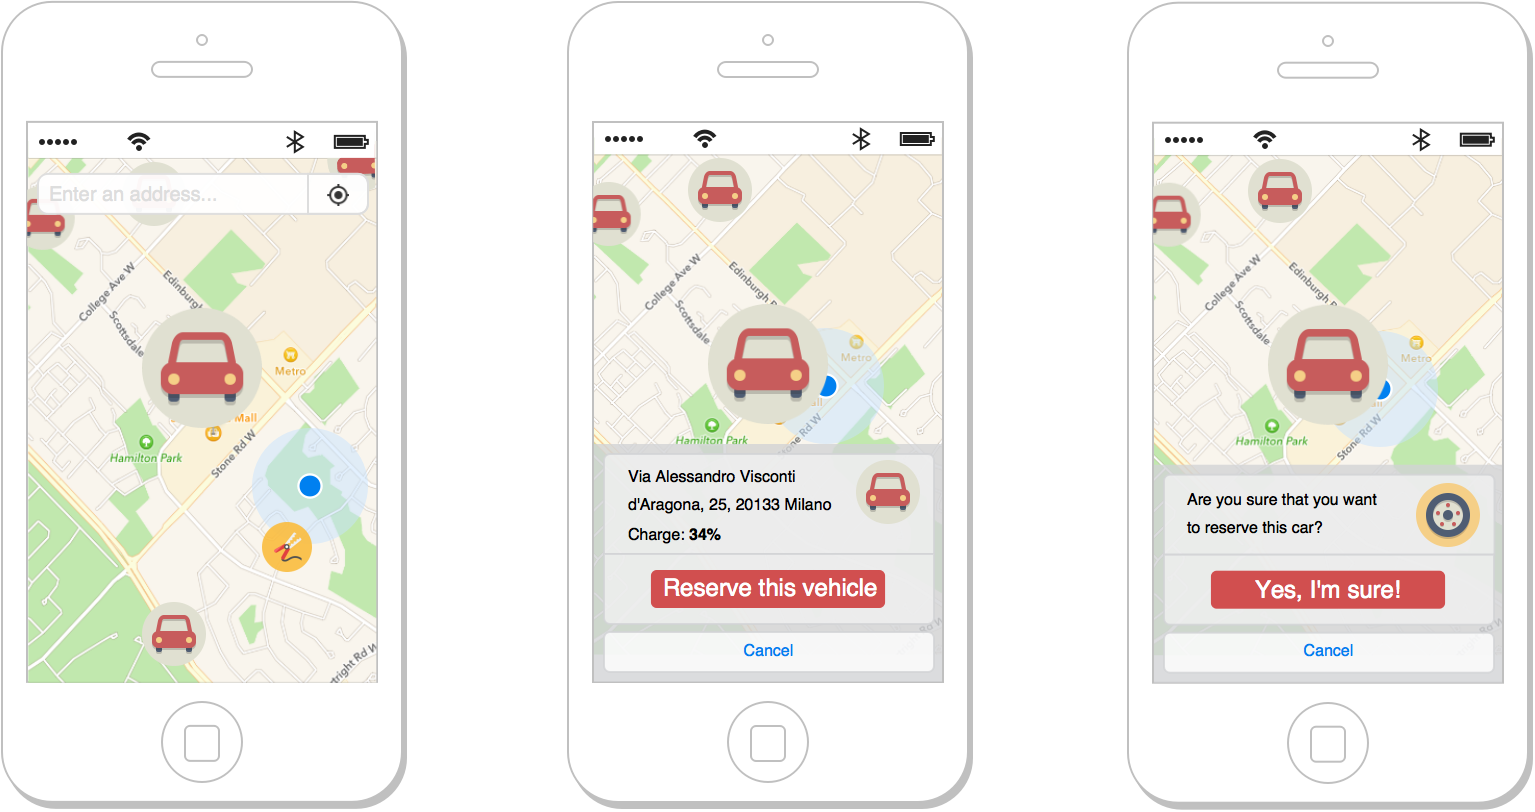
\includegraphics[width=1\textwidth]{/RASD/System_Functions/create_reservation_mockup}\\
%  \vspace{0.4cm}
%  %\caption{Mockup for the login mobile page} 
%  \label{fig:create_reservation_mockup} 
%\end{figure}
%% maybe home page mockup here 


\subsubsection{Use-case table}
\begin{center}
  \begin{tabular}{ l | p{10cm} }
    \hline
    Actors & User\\ \hline
    Goal & G\ref{itm:goal-payment}\\ \hline % To add a specific goal????
    Entry conditions & \begin{itemize}
			\item The User finishes his ride.
			\item The system is calculing the final charge

\end{itemize}  \\ \hline
  Flow of events &
\begin{itemize}
\item The system checks if one discount or one fee have to be apply to the final charge.
\item The system send a notification to the User.
\end{itemize} \\ \hline
    Exit conditions &
\begin{itemize}
	\item A possible modification of the final charge.
  \item The User has to do the payment now, as show in the "Charge ride" function.
\end{itemize}  \\ \hline
  Exceptions & 
%\begin{itemize}
%\item The User has already reserved a car.

%\item 
The system is not able to complete the operation due to some internal issues or connection broken (the system signals a ConnectionFailure).%volendo si possono modificare i nomi delle eccezzioni.
%\end{itemize} 
\\ \hline
  \end{tabular}
\end{center}


\subsubsection{Sequence diagram}
\begin{figure}[!ht]
  \centering
  \vspace{0.2cm}
  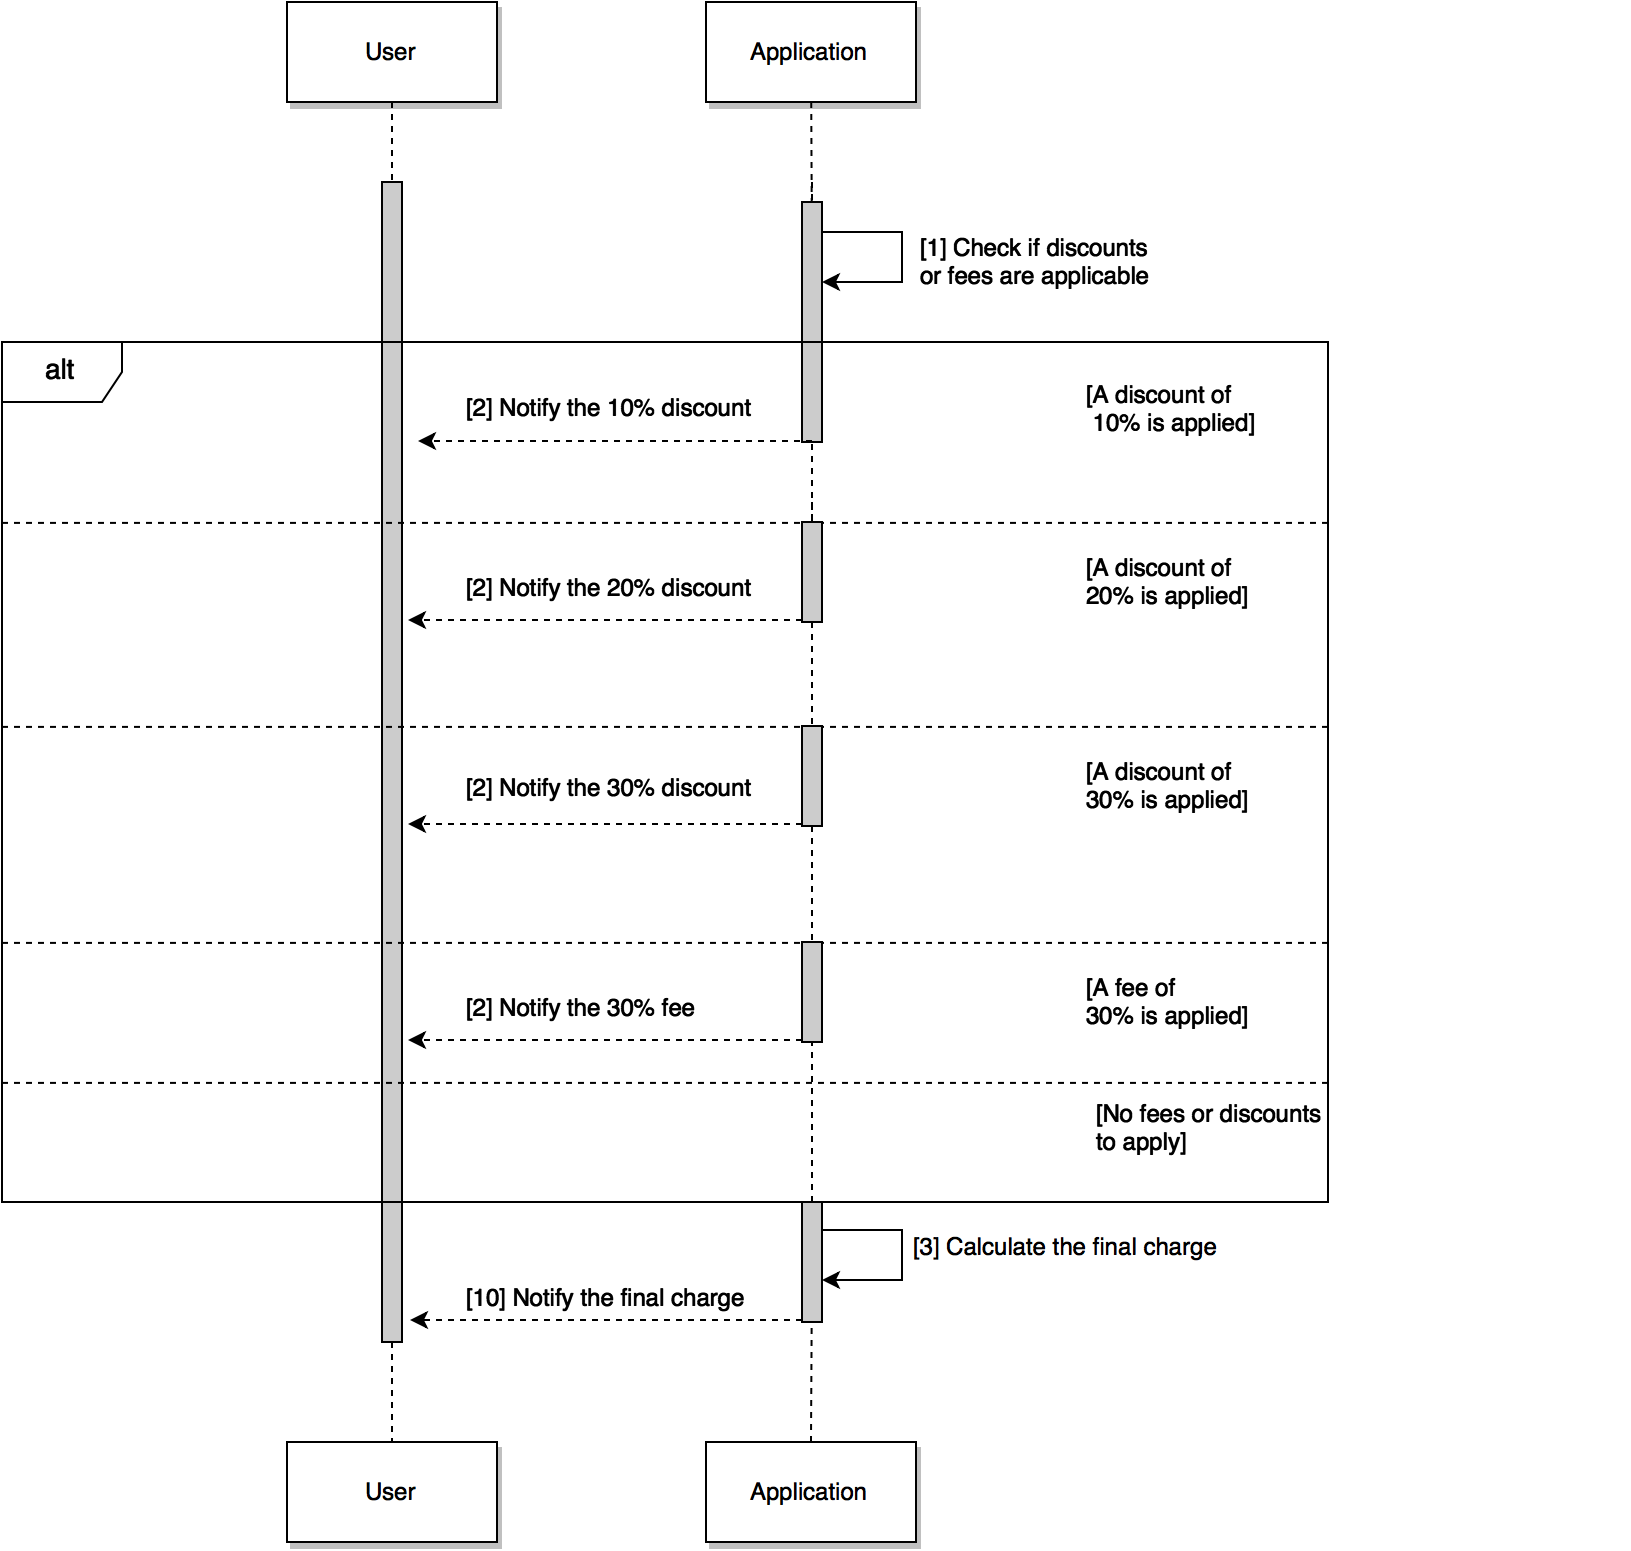
\includegraphics[width=1.2\textwidth]{/RASD/System_Functions/discountsandfees_sequence}\\
  \vspace{0.1cm}
  %\caption{Sequence diagram for the login procedure} 
  \label{fig:discountsandfees_sequence} 
\end{figure}

